\documentclass[12pt,letterpaper]{article}
\usepackage[utf8]{inputenc}
\usepackage[T1]{fontenc}
\usepackage[spanish,es-nodecimaldot]{babel}
\addto\captionsspanish{\renewcommand{\tablename}{Tabla}}
\usepackage{newtxtext,newtxmath}
\usepackage[margin=1in,headheight=15pt]{geometry}
\usepackage{setspace,graphicx,booktabs,tabularx,float,caption,fancyhdr,xurl,hyperref,titlesec}
\hypersetup{hidelinks}\urlstyle{same}
\doublespacing\setlength{\parindent}{0.5in}\setlength{\parskip}{0pt}
\setcounter{secnumdepth}{0}
\titleformat{\section}{\normalfont\bfseries\centering}{}{0pt}{}
\titlespacing*{\section}{0pt}{1em}{0pt}
\captionsetup[table]{justification=raggedright,singlelinecheck=false,labelsep=newline,labelfont=bf,textfont=it}
\pagestyle{fancy}\fancyhf{}\rhead{\thepage}\renewcommand{\headrulewidth}{0pt}
\fancypagestyle{plain}{\fancyhf{}\rhead{\thepage}\renewcommand{\headrulewidth}{0pt}}
\newcommand{\refapa}[1]{\par\noindent\hangindent=0.5in\hangafter=1 #1\par}
\newcommand{\notfig}[1]{\par\noindent\small\textit{Nota.} #1\par\normalsize}
\begin{document}\raggedright
\begin{titlepage}\thispagestyle{fancy}\begin{center}
\vspace*{1in}{\bfseries Diagnóstico y tratamiento de una fotografía con sombra intensa\par}
\vspace{1\baselineskip}
Karen Sofía Delgado Calderon\par
Especialización en Inteligencia Artificial\par
Universidad de Cundinamarca\par
604011 -- Percepción Computacional\par
R2-A2-S8S9 -- Informe de resultados de tratamiento de imagen\par
18 de octubre de 2026\par
\end{center}\vfill\end{titlepage}\setcounter{page}{2}

\begin{center}\textbf{Diagnóstico y tratamiento de una fotografía con sombra intensa}\end{center}
\section{Problema y objetivo}
Las condiciones de captura pueden impedir que una imagen conserve rasgos útiles para la percepción computacional. En este ejercicio, el mismo elefante de peluche aparece en cuatro fotografías: una referencia bien iluminada, dos capturas con iluminación desigual y una afectada por movimiento. La tarea consistió en diagnosticar estas diferencias, seleccionar una imagen problemática y probar una corrección proporcionada al defecto encontrado. No se buscó que una transformación hiciera idénticas fotografías tomadas desde encuadres distintos. La consigna del curso pide vincular el problema observado, la decisión técnica y la evaluación del resultado (Universidad de Cundinamarca, s. f.).

\section{Material y procedimiento}
Se trabajó con las cuatro imágenes suministradas para esta actividad. Las tres primeras miden $1200\times1600$ píxeles; la cuarta, $900\times1600$. Por inspección, la segunda combina zonas de sombra y una fuente de luz inferior; en la tercera, una sombra más marcada atraviesa la parte superior del rostro y reduce la visibilidad de un ojo. La cuarta presenta un barrido compatible con movimiento durante la exposición. No se dispone de ajustes de cámara ni de mediciones de iluminación, de modo que estas descripciones se limitan a lo observable en los archivos. El cambio de encuadre y de resolución de la cuarta foto impide interpretarla como una réplica píxel a píxel de la referencia.

El script \texttt{analisis\_tratamiento.py} lee los originales con OpenCV y detiene la ejecución si falta algún archivo. Para cada fotografía calcula la media de luminancia en escala de grises, su desviación estándar, el porcentaje de píxeles con intensidad menor que 50, la varianza del Laplaciano y la proporción de bordes detectados por Canny con umbrales 100 y 200. También exporta un panel de las cuatro capturas y un archivo CSV con las cifras. Se ejecutó con Python 3.14.7, OpenCV 5.0.0 y NumPy 2.5.2. La varianza del Laplaciano es una pista de cambios locales de intensidad, no una calificación universal de nitidez: la textura y el ruido pueden elevarla (OpenCV, s. f.-b).

\clearpage
\begin{figure}[H]
\noindent\textbf{Figura 1}\par
\noindent\textit{Cuatro capturas del mismo elefante de peluche}\par
\centering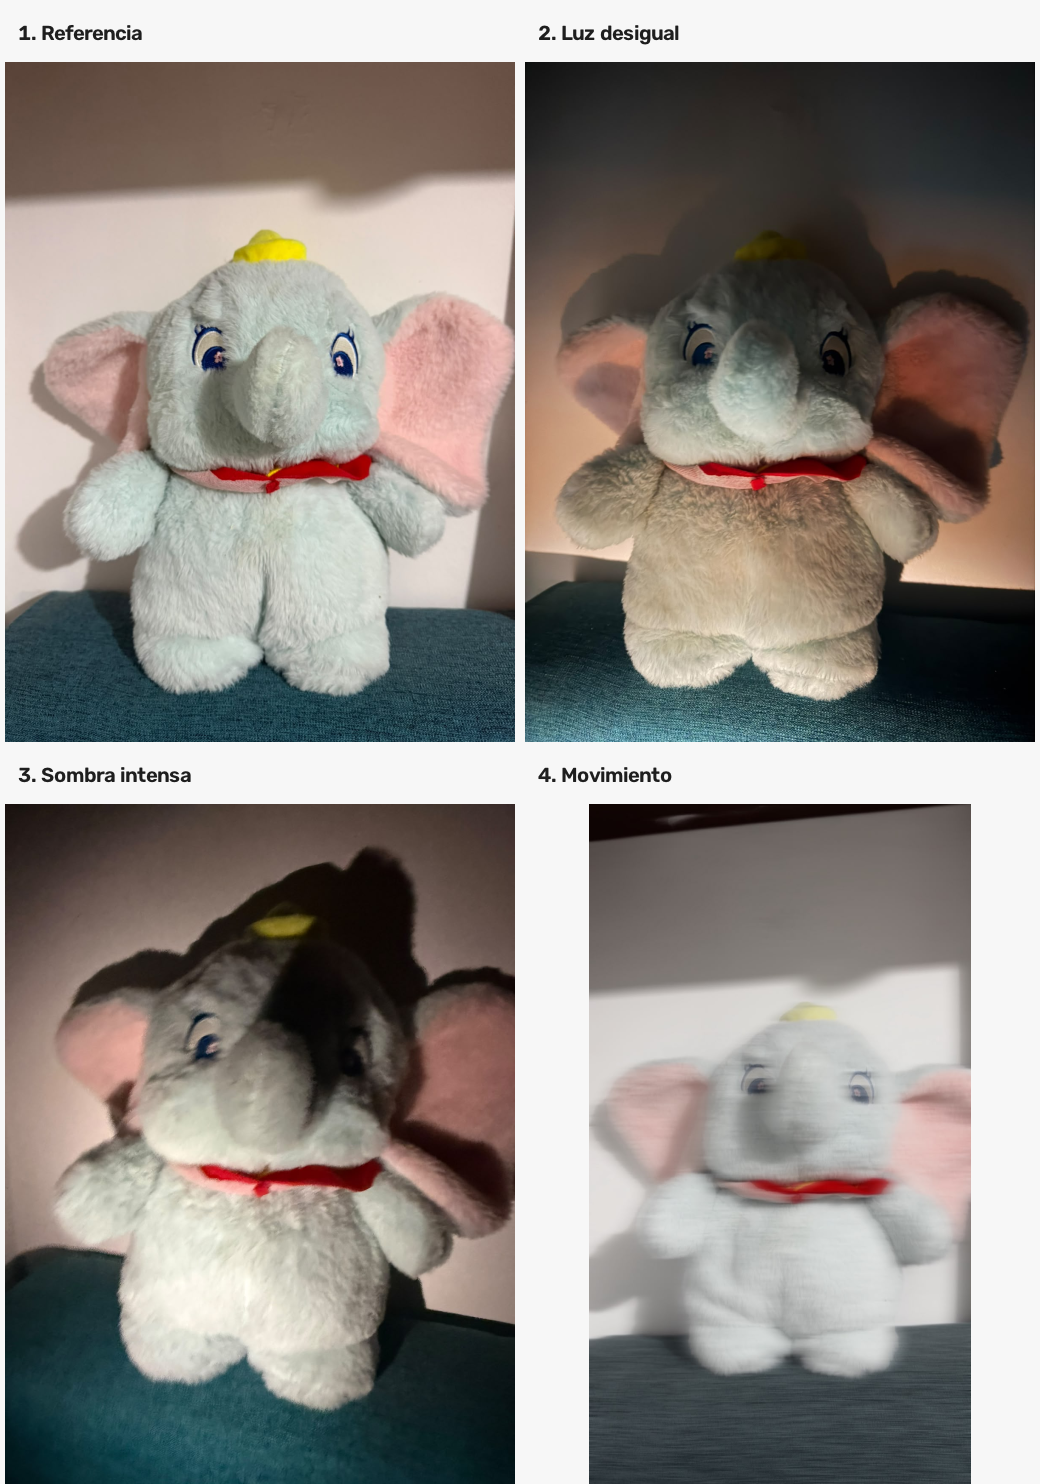
\includegraphics[width=0.78\textwidth,height=0.76\textheight,keepaspectratio]{resultados/cuatro_capturas.png}
\notfig{Panel elaborado a partir de las fotografías suministradas para el trabajo de Karen. Los rótulos describen condiciones visibles, no parámetros de cámara verificados.}
\end{figure}

\clearpage
\section{Diagnóstico y elección de la imagen}
La Tabla~\ref{tab:diagnostico} resume medidas de las imágenes completas. La referencia tuvo luminancia media de 147.48 y 4.59\% de píxeles bajo el umbral 50. La captura con luz desigual bajó a 83.79 y 37.13\%; la foto de sombra intensa registró 99.98 y 29.35\%. Aunque la segunda es más oscura globalmente, la tercera oculta una zona especialmente importante del rostro. Por eso se eligió la tercera: la decisión depende de \emph{dónde} cae la sombra y no solo del promedio de la imagen. La captura con movimiento muestra solo 0.04\% de bordes Canny frente al 2.70\% de la referencia. No se eligió para el tratamiento porque un realce de contraste no recuperaría de manera fiable los detalles barridos.

\begin{table}[H]
\caption{Diagnóstico cuantitativo de las cuatro capturas}\label{tab:diagnostico}
\small\begin{tabularx}{\textwidth}{Xrrrr}
\toprule
Captura & Media & Oscuros (\%) & Var. Lap. & Bordes (\%)\\
\midrule
Referencia & 147.48 & 4.59 & 1143.79 & 2.70\\
Luz desigual & 83.79 & 37.13 & 1865.00 & 2.63\\
Sombra intensa & 99.98 & 29.35 & 142.14 & 0.34\\
Movimiento & 140.60 & 3.55 & 117.74 & 0.04\\
\bottomrule
\end{tabularx}\normalsize
\par\noindent\small\textit{Nota.} Media: intensidad de gris en escala 0--255. Oscuros: píxeles menores que 50. Var. Lap.: varianza del Laplaciano, dependiente de textura y escala. Los porcentajes de bordes usan el mismo umbral Canny; la foto de movimiento tiene menor ancho.\normalsize
\end{table}

\section{Tratamiento justificado}
Se aplicó ecualización adaptativa de histograma con límite de contraste (CLAHE) al canal de luminancia $L$ en el espacio de color Lab; los canales cromáticos se conservaron. El parámetro \texttt{clipLimit} fue 1.8 y la retícula fue de $8\times8$ bloques. Esta elección apunta a la pérdida local de visibilidad bajo la sombra y limita la amplificación extrema del contraste. OpenCV describe el límite de contraste como una medida para contener la amplificación de ruido en ecualización adaptativa (OpenCV, s. f.-a). No se aplicó un filtro de nitidez a la imagen movida ni una cadena indiscriminada de transformaciones. El archivo \texttt{sombra\_tratada.png} es una copia derivada; los originales permanecen intactos.

\section{Resultados y evaluación}
Para estudiar el área relevante, el script usa un recorte fijo del rostro de la tercera fotografía, desde $(x,y)=(300,300)$ hasta $(950,900)$. Se compara ese mismo recorte antes y después; no se comparan directamente píxeles con la referencia porque el encuadre cambió. En la imagen completa tratada, los píxeles oscuros bajaron de 29.35\% a 24.59\% y la luminancia media subió de 99.98 a 105.90. En el rostro, los oscuros pasaron de 36.66\% a 33.48\% y la media de 96.16 a 100.52 (Tabla~\ref{tab:resultado}). La proporción de bordes detectados aumentó, pero ese cambio puede incluir textura y grano realzados; no prueba por sí mismo mayor exactitud de reconocimiento.

\begin{table}[H]
\caption{Comparación de la fotografía con sombra antes y después de CLAHE}\label{tab:resultado}
\small\begin{tabularx}{\textwidth}{Xrrrr}
\toprule
Región y estado & Media & Oscuros (\%) & Var. Lap. & Bordes (\%)\\
\midrule
Completa, antes & 99.98 & 29.35 & 142.14 & 0.34\\
Completa, después & 105.90 & 24.59 & 419.22 & 0.84\\
Rostro, antes & 96.16 & 36.66 & 166.62 & 0.54\\
Rostro, después & 100.52 & 33.48 & 372.69 & 0.98\\
\bottomrule
\end{tabularx}\normalsize
\par\noindent\small\textit{Nota.} El rostro corresponde al mismo recorte de $650\times600$ píxeles en las versiones antes y después. Los indicadores no constituyen una prueba de desempeño de un clasificador.\normalsize
\end{table}

\begin{figure}[H]
\noindent\textbf{Figura 2}\par
\noindent\textit{Referencia visual, fotografía con sombra y versión tratada}\par
\centering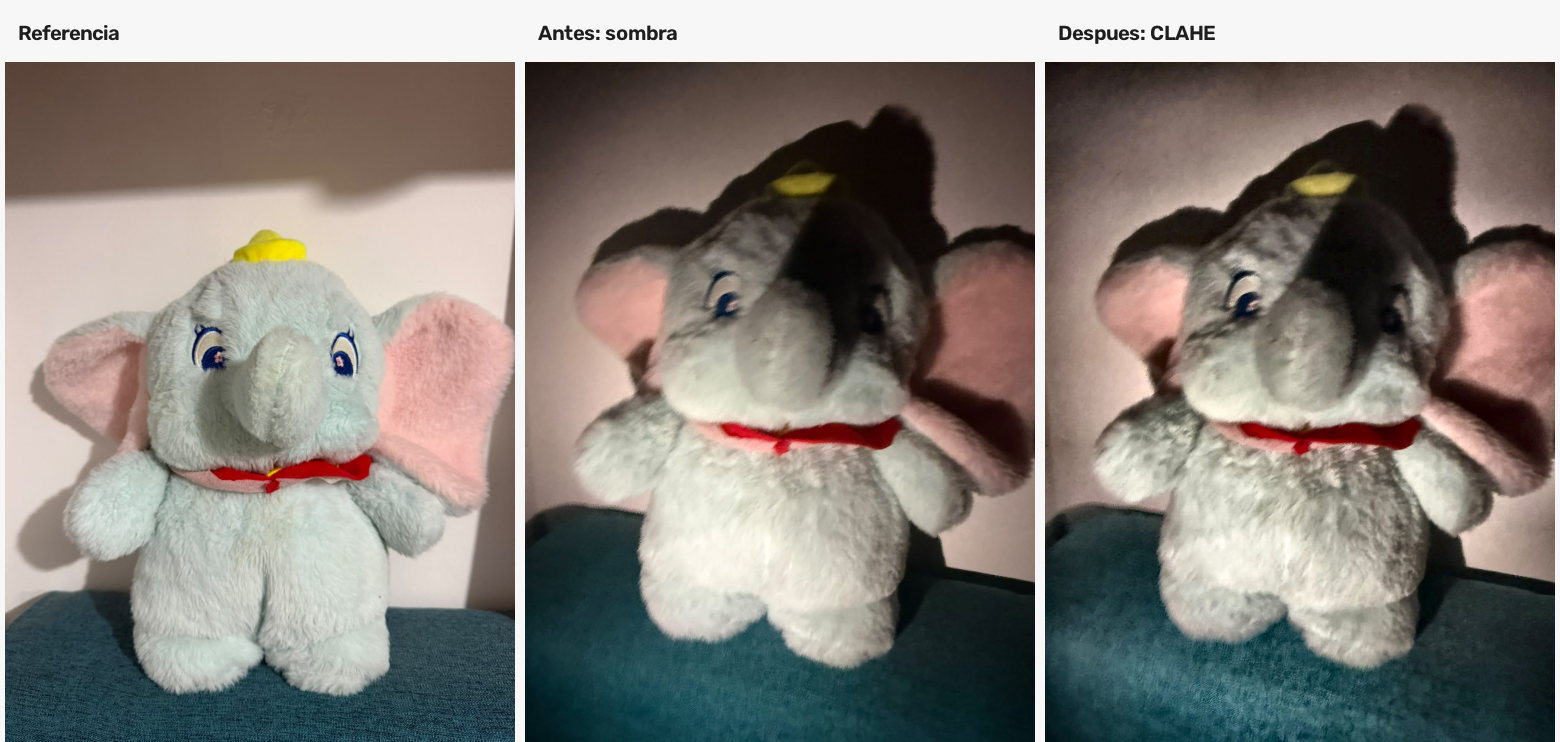
\includegraphics[width=\textwidth,height=0.41\textheight,keepaspectratio]{resultados/comparacion_tratamiento.png}
\notfig{La fotografía de referencia permite apreciar el objeto, pero no está alineada píxel a píxel con la captura intervenida. La imagen tratada se generó con el script adjunto.}
\end{figure}

\section{Discusión y conclusiones}
El tratamiento hace algo más visibles partes del peluche situadas alrededor de la sombra, pero no elimina la oclusión lumínica profunda del ojo ni reproduce la iluminación uniforme de la referencia. El aumento de varianza del Laplaciano y de bordes, junto con la inspección de la Figura~2, sugiere realce de textura; no debe confundirse con recuperación demostrada de información perdida. La mejora cuantitativa en el rostro fue moderada: 3.18 puntos porcentuales menos de píxeles oscuros. Si la tarea posterior requiere reconocer rasgos finos de ambos ojos, volver a capturar con iluminación frontal estable sería más defendible que aumentar todavía más el contraste.

Este caso muestra que la elección técnica se decide por el rasgo que necesita el sistema, no por la métrica global más llamativa. La segunda fotografía era la más oscura en promedio, mientras que la tercera bloqueaba visualmente una región crítica. CLAHE fue una intervención reproducible y acotada para esa tercera imagen. Queda como límite no haber evaluado un detector o clasificador posterior ni disponer de una toma idénticamente encuadrada como verdad de referencia; por ello la conclusión se restringe a la visibilidad observada y a las métricas descriptivas reportadas.

\section{Disponibilidad del código}
El código reproducible, las fotografías originales y las salidas se organizan en el repositorio público de la cuenta \texttt{sofiadelcal}: \url{https://github.com/sofiadelcal/karen-tratamiento-imagen}. El informe identifica a Karen como autora del trabajo, aunque el repositorio esté alojado en otra cuenta por indicación del usuario.

\newpage
\section{Referencias}
\refapa{OpenCV. (s. f.-a). \textit{Histograms -- 2: Histogram equalization}. \url{https://docs.opencv.org/4.x/d5/daf/tutorial_py_histogram_equalization.html}}
\refapa{OpenCV. (s. f.-b). \textit{Laplace operator}. \url{https://docs.opencv.org/4.x/d5/db5/tutorial_laplace_operator.html}}
\refapa{Universidad de Cundinamarca. (s. f.). \textit{R2-A2-S8S9: Informe de resultados de tratamiento de imagen} [Consigna del curso 604011, Percepción Computacional]. Aula de Posgrado.}
\end{document}
